% !TeX spellcheck = en_US
% !TeX encoding = UTF-8 

\documentclass[14pt,a4paper]{extarticle}

\usepackage[english]{babel}
\usepackage[utf8]{inputenc}
\usepackage{setspace} 
\usepackage[a4paper,
			left=30mm,
			right=10mm,
			top=20mm,
			bottom=20mm]{geometry}
\usepackage{amsmath}
\usepackage{amssymb}
\usepackage{amsthm}
\usepackage{graphicx} 
\usepackage{cite}
\usepackage{subfigure}
\usepackage{subcaption}
\usepackage{kprjHSE} 
\usepackage{listings}
\usepackage{xcolor,tabularray}
\usepackage{courier}
\usepackage{hyperref}
\hypersetup{
	colorlinks=true,
	linkcolor=black,
	citecolor=black,
	filecolor=black,      
	urlcolor=blue,
}

\lstset{
	frame=single,
	basicstyle=\ttfamily,
	breaklines=true,
	tabsize=4
}

\homeworkHSE

\FirstAuthor{M.D.~Kirdin}
\SecondAuthor{V.M.~Pendishchuk}
\discipline{Basic Methods of Data Analysis}
\faculty{Faculty of Computer Science}
\chair{School of Data Analysis and Artificial Intelligence}
\chief{B.G.~Mirkin}
\workyear{2024}

\onehalfspacing

\begin{document}
	
	\tableofcontents
	
	\section{Data}
	
	
	\section{Correlation coefficient}
	
	To understand which pair of features is the best for constructing a linear regression on, we have to take into account their distributions. As shown on \figref{fig:pairplot}, there are several features of interest: "x", "y", "z", "carat" and "price". Features "x", "y" and "z", with the exception of some outliers, are distributed in a linear pattern and their distributions wrt "carat" look like polynomial functions. This is an expected behavior, since "carat" is roughly the product of "x", "y", "z", which are linearly distributed with each other, and diamond density. 
	
	\begin{figure}[hbtp]
		\centering
		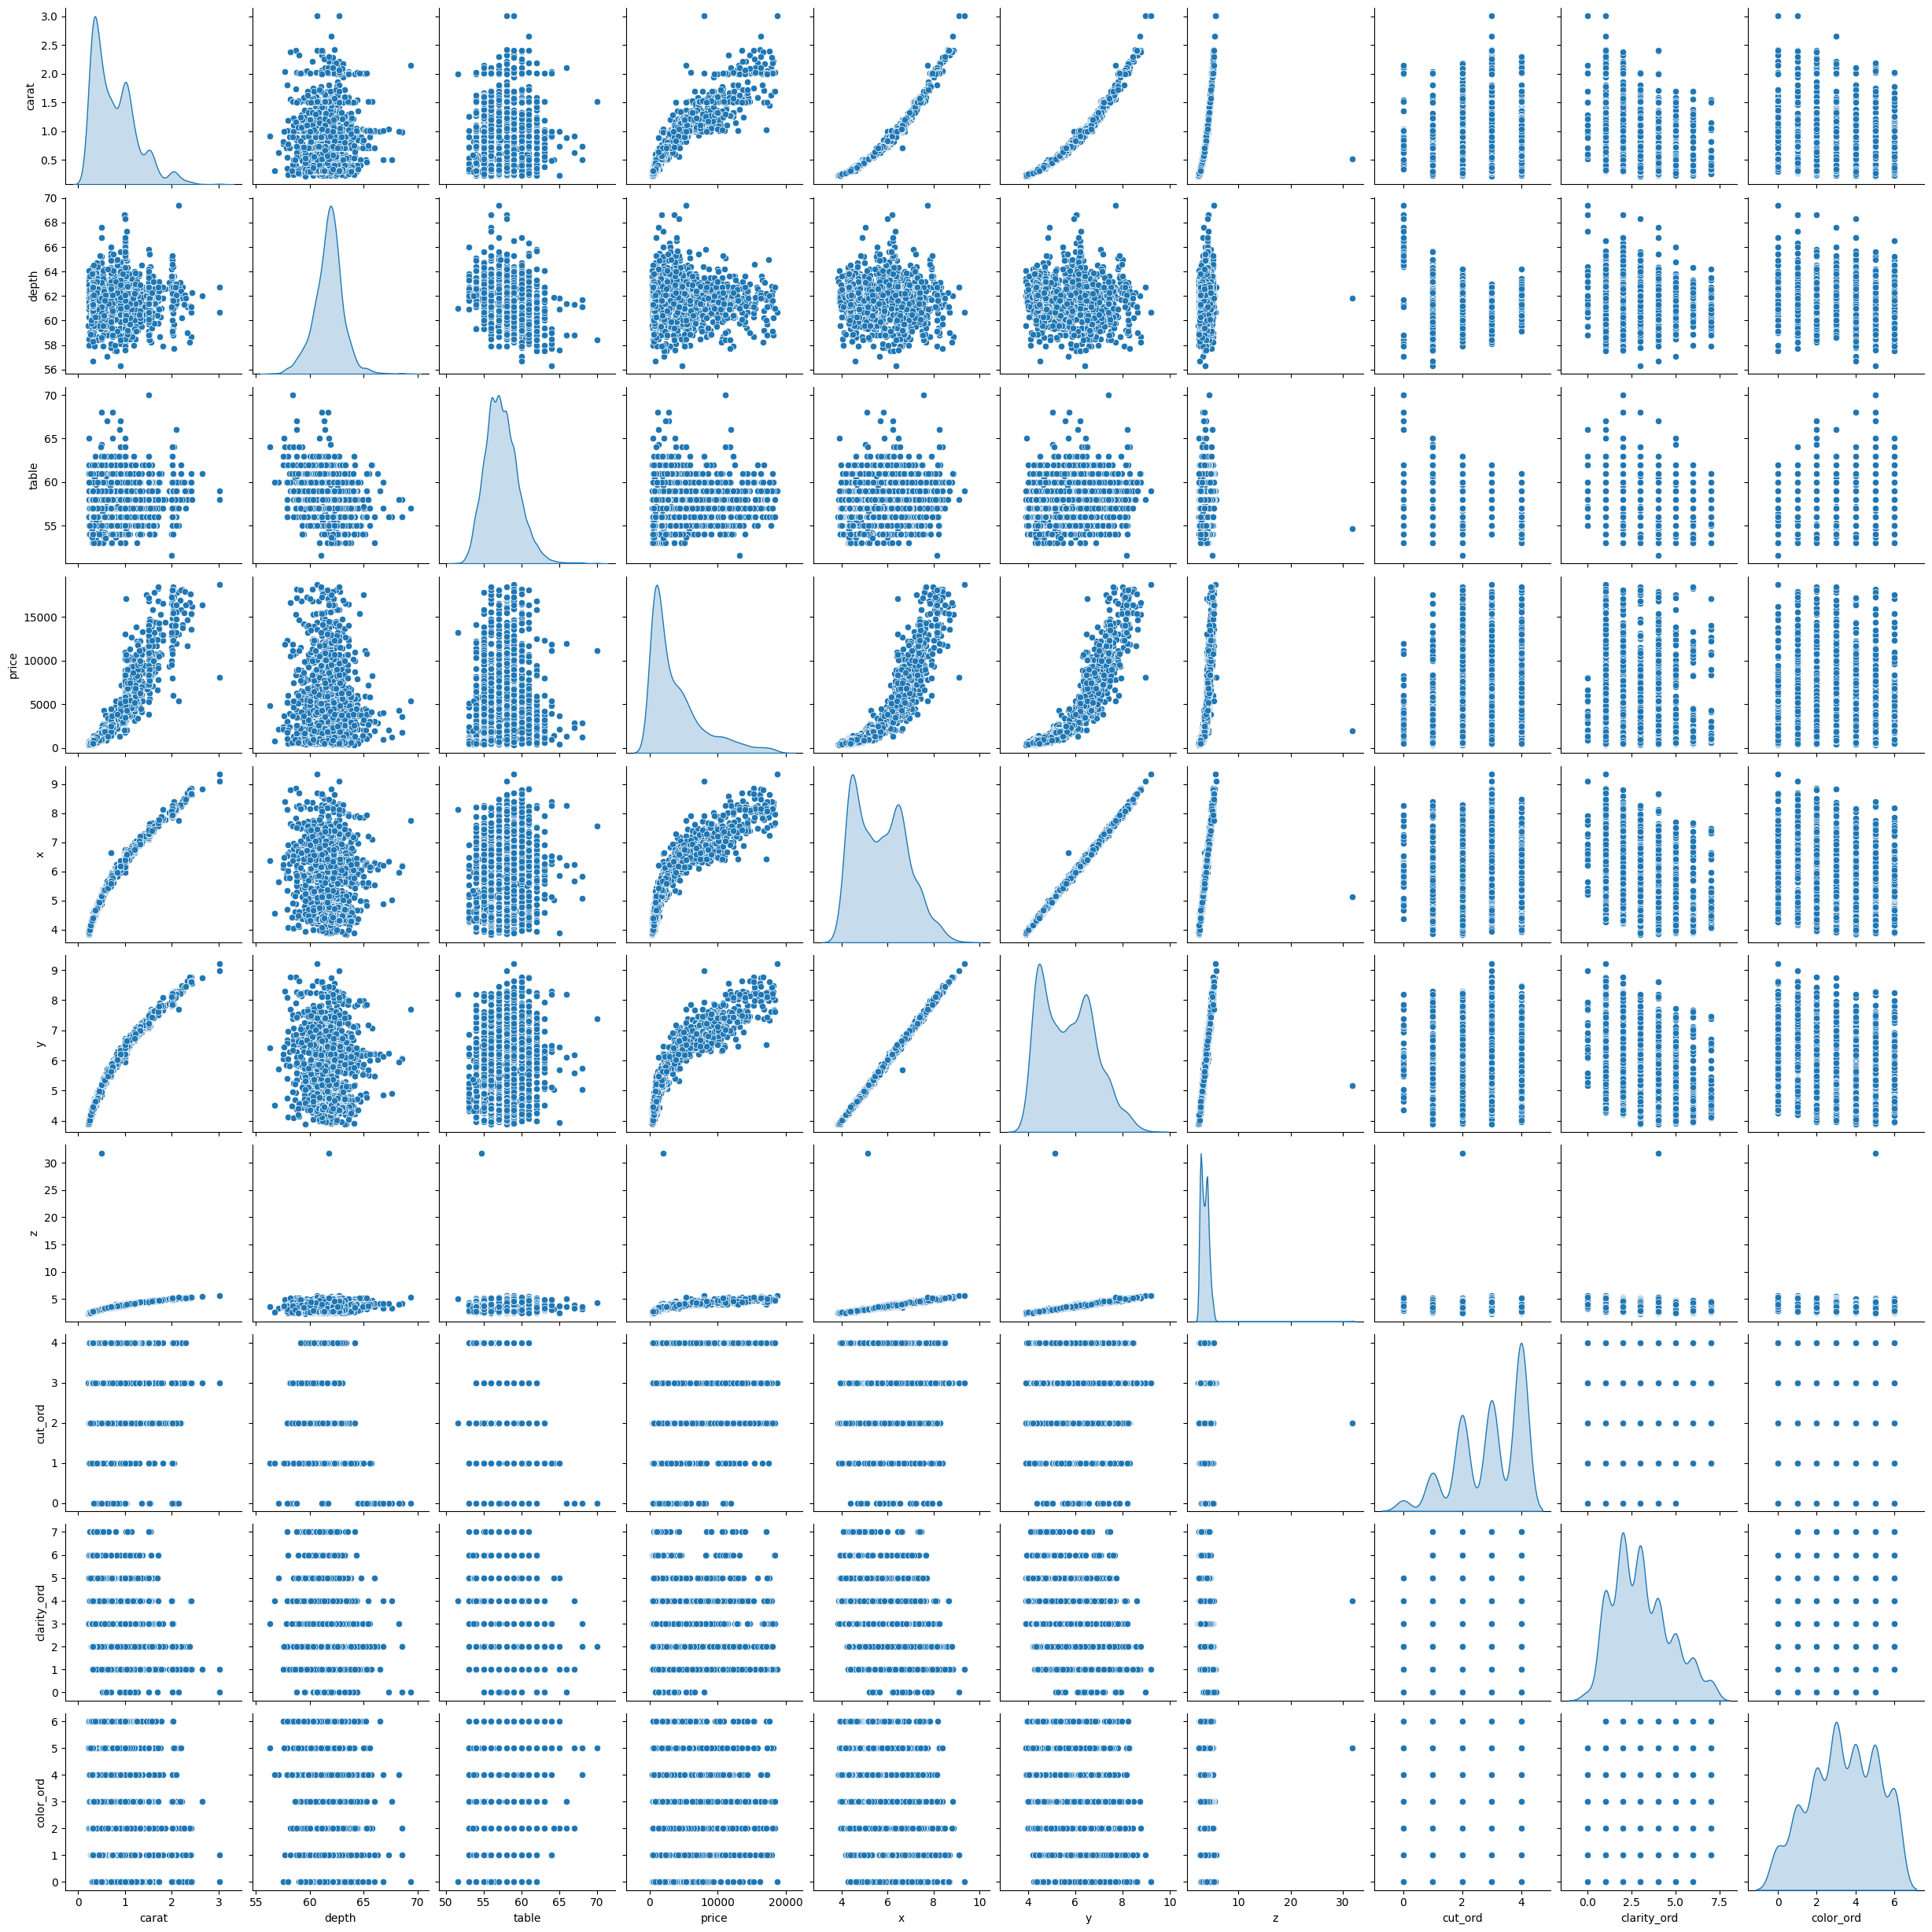
\includegraphics[width=.95\textwidth]{media/pairplot.png}
		\caption{Pairwise scatter plots of all the features in data}
		\label{fig:pairplot}
	\end{figure}
	
	\newpage
	
	In this task we will consider the pair "carat" and "price", because their distribution is not as trivial as those of diamonds' physical dimensions wrt each other or their mass (\figref{fig:caratVprice}).
	
	\begin{figure}[hbtp]
		\centering
		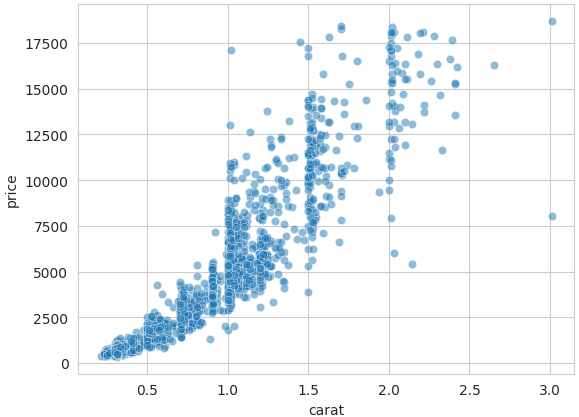
\includegraphics[width=.8\textwidth]{media/caratVprice.png}
		\caption{Distribution "carat" and "price" wrt each other}
		\label{fig:caratVprice}
	\end{figure}
	
	First, a regular linear regression of "price" over "carat" was constructed. As shown on \figref{fig:caratVpriceReg}, this line has a positive slope, hence the diamond's price tends to positively correlate with its mass, which is to be expected. Next, the correlation and $R^2$ coefficient, also known as \textit{the coefficient of determination}, were computed:
	\[\rho = 0.9240,\, R^2 = 0.8537.\]
	Since $R^2$ coefficient is the proportion of variance of the target feature taken into account by linear regression, in our case  $85.37\%$ of "price" variance is taken into account.
	
	After that, a set 
	\[x=\begin{pmatrix}
			0.3000 & 863\\
			0.3100 & 788\\
			0.4000 & 662\\ 
			2.0100 & 17078
		\end{pmatrix}\]
	of four random pairs of "carat" and "price" values was chosen to compare the predicted and true "price" values. To do this, the percentile deviations were found:
	\begin{multline*}
	\Delta{}y_{\text{true}} = \left(89.9245\%,\, 79.1276\%,\, -30.2385\%,\, 21.8683\%\right)^T,\\ \Delta{}y_{\text{pred}}=\left(892.5046\%,\, 379.1018\%,\, -23.2178\%,\, 27.9890\%\right)^T,
	\end{multline*}
	where $\Delta{}y_{\text{true}}$ is relative deviation of predicted from true values and $\Delta{}y_{\text{pred}}$ is the other way round. From this we can conclude that the regression line tends to underestimate the price of diamonds with lower mass.
	
	\begin{figure}[hbtp]
		\centering
		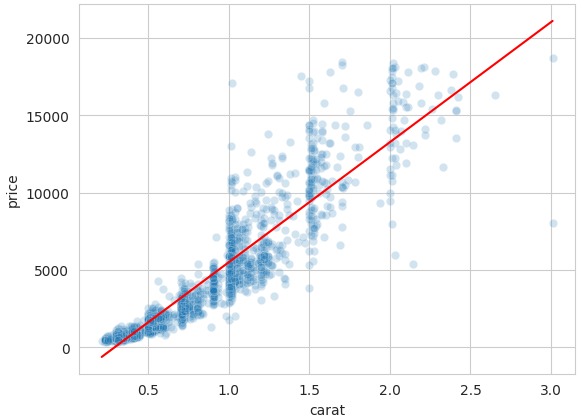
\includegraphics[width=.8\textwidth]{media/caratVpriceReg.png}
		\caption{Linear regression of "price" over "carat"}
		\label{fig:caratVpriceReg}
	\end{figure}
	
	Finally, mean absolute percentile error(MAPE) relative to both true and predicted over the whole data was considered in order to measure the mean deviation of the data from the predictor line and vice versa:
	\[\text{MAPE}_{\text{true}}= 39.2063\%,\, \text{MAPE}_{\text{pred}}=121.4897\%.\]
	These values indicate that, similarly to the previous case, regression on this pair features tends to underestimate the "price" feature. There is also another interpretation: $\text{MAPE}_{\text{true}}$ is data analysis(DA) view on MAPE, while $\text{MAPE}_{\text{pred}}$ is machine learning(ML) view on MAPE; hence, while in terms of DA the line we constructed is good, while the opposite is true in terms of ML.
	
	We also tried polynomial regression with a third degree polynomial, as seen on \figref{fig:caratVpriceRegAlt}. This resulting in following MAPE values:
	\[\text{MAPE}_{\text{true}}= 39.2063\%,\, \text{MAPE}_{\text{pred}}=37.0984\%.\]
	This indicates that the polynomial curve uses more data and does not underestimate the price.
	
	\begin{figure}[hbtp]
		\centering
		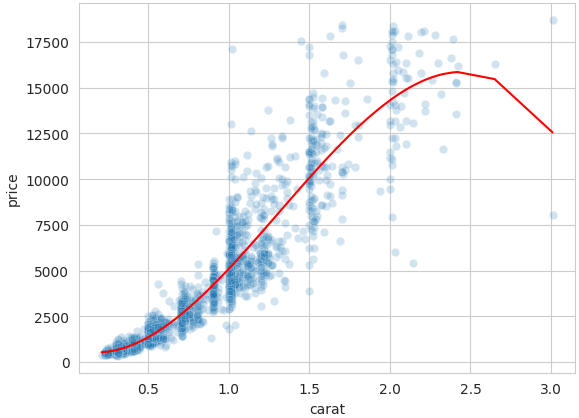
\includegraphics[width=.8\textwidth]{media/caratVpriceRegAlt.png}
		\caption{Polynomial regression of "price" over "carat"}
		\label{fig:caratVpriceRegAlt}
	\end{figure}
	
	\section{Cluster analysis and cluster interpretation}
	
	To understand the general pricing patterns a following subset of features was explored via K-Means algorithm:
	\begin{itemize}
		\item "depth";
		\item "table";
		\item "carat";
		\item "price".
	\end{itemize}
	These features denote the physical parameters of a diamond and were scaled to have normal distribution before the clustering algorithm was applied to them. 
	
	Then, using the build-in K-Means algorithm with 4 and 7 clusters were applied to the data. It was initialized to start with twelve sets of random centers for each number of clusters used. Algorithm's performance was measured with inertia metric:
	\[L = \sum\limits_{k=1}^{K}\sum\limits_{i\in S_{k}}\sum\limits_{v\in V} \left(y_{iv} - c_{kv}\right)^2,\]
	where $K$ is the number of clusters;
	
	$S_k$ is the number of objects in $k$-th cluster;
	
	$V$ is the set of features;
	
	$y_{iv}$ is value of feature $v$ of the $i$-th object from cluster $k$;
	
	$c_{kv}$ is value of feature $v$ of the center of cluster $k$.
	
	After the evaluation, for each number of clusters the best-performing cluster set was chosen for further analysis. On those the absolute and relative deviations from grand mean for each feature were calculated: 
	\[d_{abs}=(c_{kv}-c_{v}),\, d_{rel}=\dfrac{c_{kv}-c_{v}}{c_v}\cdot100\%.\]
	For each cluster in each table deviations in a feature of more than 30\% were marked with green(positive deviations) and red(negative deviation) backgrounds. 
	
	\begin{center}
		\noindent \textbf{Table 1.} Best set for K-Means with 4 clusters
		\begin{tblr}{width=\linewidth,
			vline{0,1-6}={1-19}{0.5pt},
			hline{0,1-19}={1-6}{0.5pt}}
			 & \textbf{depth} & \textbf{table} & \textbf{carat} & \textbf{price}\\
			 
			grand mean & 61.7409 & 57.3868 & 0.7865 & 3858.1980\\
			 
			\SetCell[r=1, c=5]{c}{\textbf{cluster 1 (234 instances)}}\\
			center & 61.4547 & 58.0838 & \SetCell{green8}1.6865 & \SetCell{green8}12463.5812\\
			grand mean devation & -0.2861 & 0.6970 & \SetCell{green8}0.9000 & \SetCell{green8}8605.3832\\
			rel. grand mean deviation & -0.46\% & 1.21\% & \SetCell{green8}114.44\% & \SetCell{green8}223.04\%\\
			
			\SetCell[r=1, c=5]{c}{\textbf{cluster 2 (854 instances)}}\\
			center & 62.0034 & 56.1681 & \SetCell{red9}0.4438 & \SetCell{red8}1276.4660\\
			grand mean devation & 0.2625 & -1.2187 & \SetCell{red9}-0.3427 & \SetCell{red8}-2581.7320\\
			rel. grand mean deviation & 0.43\% & -2.12\% & \SetCell{red9}-43.57\% & \SetCell{red8}-66.92\%\\
			
			\SetCell[r=1, c=5]{c}{\textbf{cluster 3 (512 instances)}}\\
			center & 62.5969 & 57.3387 & \SetCell{green9}1.0456 & \SetCell{green9}5258.8340\\
			grand mean devation & 0.8560 & -0.0481 & \SetCell{green9}0.2592 & \SetCell{green9}1400.6360\\
			rel. grand mean deviation & 1.39\% & -0.08\% & \SetCell{green9}32.95\% & \SetCell{green9}36.30\%\\
			
			\SetCell[r=1, c=5]{c}{\textbf{cluster 4 (400 instances)}}\\
			center & 60.2520 & 59.6425 & 0.6599 & \SetCell{red9}2543.2325\\
			grand mean devation & -1.4889 & 2.2557 & -0.1266 & \SetCell{red9}-1314.9655\\
			rel. grand mean deviation & -2.41\% & 3.93\% & -16.10\% & \SetCell{red9}-34.08\%
		\end{tblr}
	\end{center}
	
	According to the table 1, those four clusters correspond to extremely valuable, extremely cheap, moderately valuable and moderately cheap diamonds respectively. Interestingly, "depth" and "table" do not deviate that much from their respective grand means and do not correlate with neither "price" nor "carat".
	
	Similar conclusion can be made for the case with 7 clusters. They correspond to various "price" and "mass" ranges with clusters in similar range being divided based on their "depth" and "table" deviations.
	\newpage
	\begin{center}
		\noindent \textbf{Table 2.} Best set for K-Means with 7 clusters
		\begin{tblr}{width=\linewidth,
				vline{0,1-6}={1-27}{0.5pt},
				hline{0,1-27}={1-6}{0.5pt}}
			& \textbf{depth} & \textbf{table} & \textbf{carat} & \textbf{price}\\
			
			grand mean & 61.7409 & 57.3868 & 0.7865 & 3858.1980\\
			
			\SetCell[r=1, c=5]{c}{\textbf{cluster 1 (193 instances)}}\\
			center & 61.5523 & 58.2466 & \SetCell{green8}1.7496 & \SetCell{green8}13071.0829\\
			grand mean devation & -0.1885 & 0.8598 & \SetCell{green8}0.9631 & \SetCell{green8}9212.8849\\
			rel. grand mean deviation & -0.31\% & 1.50\% & \SetCell{green8}122.46\% & \SetCell{green8}238.79\%\\
			
			\SetCell[r=1, c=5]{c}{\textbf{cluster 2 (290 instances)}}\\
			center & 60.5655 & 57.3117 & \SetCell{red9}0.4779 & \SetCell{red8}1450.8103\\
			grand mean devation & -1.1753 & -0.0751 & \SetCell{red9}-0.3085 & \SetCell{red8}-2407.3877\\
			rel. grand mean deviation & -1.90\% & -0.13\% & \SetCell{red9}-39.23\% & \SetCell{red8}-62.40\%\\
			
			\SetCell[r=1, c=5]{c}{\textbf{cluster 3 (350 instances)}}\\
			center & 62.3123 & 58.0829 & \SetCell{red8}0.4388 & \SetCell{red8}1231.0829\\
			grand mean devation & 0.5714 & 0.6961 & \SetCell{red8}-0.3476 & \SetCell{red8}-2627.1151\\
			rel. grand mean deviation & 0.93\% & 1.21\% & \SetCell{red8}-44.20\% & \SetCell{red8}-68.09\%\\
			
			\SetCell[r=1, c=5]{c}{\textbf{cluster 4 (192 instances)}}\\
			center & 59.7719 & 60.8776 & 0.8353 & 3704.7188\\
			grand mean devation & -1.9690 & 3.4908 & 0.0488 & -153.4792\\
			rel. grand mean deviation & -3.19\% & 6.08\% & 6.21\% & -3.98\%\\
			
			\SetCell[r=1, c=5]{c}{\textbf{cluster 5 (184 instances)}}\\
			center & 63.7891 & 58.3761 & 1.0024 & 4422.3478\\
			grand mean devation & 2.0483 & 0.9893 & 0.2159 & 564.1498\\
			rel. grand mean deviation & 3.32\% & 1.72\% & 27.45\% & 14.62\%\\
			
			\SetCell[r=1, c=5]{c}{\textbf{cluster 6 (431 instances)}}\\
			center & 62.1624 & 55.0935 & \SetCell{red8}0.4575 & \SetCell{red8}1338.5963\\
			grand mean devation & 0.4216 & -2.2933 & \SetCell{red8}-0.3290 & \SetCell{red8}-2519.6017\\
			rel. grand mean deviation & 0.68\% & -4.00\% & \SetCell{red8}-41.83\% & \SetCell{red8}-65.31\%\\
		\end{tblr}
	\end{center}
	\newpage
	\begin{center}
		\noindent \textbf{Table 2.} Best set for K-Means with 7 clusters
		\begin{tblr}{width=\linewidth,
				vline{0,1-6}={1-27}{0.5pt},
				hline{0,1-27}={1-6}{0.5pt}}
			& \textbf{depth} & \textbf{table} & \textbf{carat} & \textbf{price}\\
			\SetCell[r=1, c=5]{c}{\textbf{cluster 7 (360 instances)}}\\
			center & 61.7317 & 56.6878 & \SetCell{green8}1.1141 & \SetCell{green8}6222.5278\\
			grand mean devation & -0.0092 & -0.6990 & \SetCell{green8}0.3277 & \SetCell{green8}2364.3298\\
			rel. grand mean deviation & -0.01\% & -1.22\% & \SetCell{green8}41.66\% & \SetCell{green8}61.28\%\\
		\end{tblr}
	\end{center}
	
	Overall, "depth" and "table" seem to have no correlation to both the diamond's price and its mass. Increasing the number of classes seems to subdivide the price ranges into smaller pieces determined by their "table" and "depth".
	
%	\def\bibindent{-0.8em}
%	\begin{thebibliography}{\kern\bibindent} \makeatletter \let\old@biblabel\@biblabel \def\@biblabel#1{\hspace{12.5 mm}\old@biblabel{#1}\kern\bibindent} \let\old@bibitem\bibitem \def\bibitem#1{\old@bibitem{#1}\leavevmode\kern-\bibindent} \makeatother
%		
%		\bibitem{glioma_classification}
%		Byun YH, Park CK. Classification and Diagnosis of Adult Glioma: A Scoping Review // Brain Neurorehabil. 2022 Nov; vol.~15(3):e23. https://doi.org/10.12786/bn.2022.15.e23
%	\end{thebibliography}
\end{document}